%%%%%%%%%%%%%%%%%%%%%%%%%%%%%%%%%%%%%%%%%
% University Assignment Title Page 
% LaTeX Template
% Version 1.0 (27/12/12)
%
% This template has been downloaded from:
% http://www.LaTeXTemplates.com
%
% Original author:
% WikiBooks (http://en.wikibooks.org/wiki/LaTeX/Title_Creation)
%
% License:
% CC BY-NC-SA 3.0 (http://creativecommons.org/licenses/by-nc-sa/3.0/)
% 
% Instructions for using this template:
% This title page is capable of being compiled as is. This is not useful for 
% including it in another document. To do this, you have two options: 
%
% 1) Copy/paste everything between \begin{document} and \end{document} 
% starting at \begin{titlepage} and paste this into another LaTeX file where you 
% want your title page.
% OR
% 2) Remove everything outside the \begin{titlepage} and \end{titlepage} and 
% move this file to the same directory as the LaTeX file you wish to add it to. 
% Then add \input{./title_page_1.tex} to your LaTeX file where you want your
% title page.
%
%%%%%%%%%%%%%%%%%%%%%%%%%%%%%%%%%%%%%%%%%
%\title{Title page with logo}
%----------------------------------------------------------------------------------------
%	PACKAGES AND OTHER DOCUMENT CONFIGURATIONS
%----------------------------------------------------------------------------------------

\documentclass[12pt]{article}
\usepackage[english]{babel}
\usepackage[utf8x]{inputenc}
\usepackage{amsmath}
\usepackage{graphicx}
\usepackage[colorinlistoftodos]{todonotes}
\usepackage{subcaption}

\begin{document}

\begin{titlepage}

\newcommand{\HRule}{\rule{\linewidth}{0.5mm}} % Defines a new command for the horizontal lines, change thickness here

\center % Center everything on the page
 
%----------------------------------------------------------------------------------------
%	HEADING SECTIONS
%----------------------------------------------------------------------------------------

% Name of your university/college
\textsc{\LARGE Instituto Superior T\'{e}cnico}\\[1.5cm]
% Major heading such as course name
\textsc{\Large ISR}\\[0.5cm]
% First Minor heading such as course title
\textsc{\large Report}\\[0.25cm]
% Second Minor heading such as course title
\textsc{\small State Of The Art Milestone}\\[0.25cm]

%----------------------------------------------------------------------------------------
%	TITLE SECTION
%----------------------------------------------------------------------------------------

\HRule \\[0.5cm]
{ \large \bfseries State Of The Art Essay: A First Approach}\\[0.25cm] % Title of your document
\HRule \\[0.5cm]
 
%----------------------------------------------------------------------------------------
%	AUTHOR SECTION
%----------------------------------------------------------------------------------------

\begin{minipage}{0.4\textwidth}
\begin{flushleft} \large
\emph{Author:}\\
Francisco Maria \textsc{Calisto} % Your name
\end{flushleft}
\end{minipage}
~
\begin{minipage}{0.4\textwidth}
\begin{flushright} \large
\emph{Coordinator:} \\
Jacinto \textsc{Peixoto} % Coordinator's Name
\end{flushright}
~
\begin{flushright} \large
\emph{Co-Coordinator:} \\
Daniel \textsc{Gon\c{c}alves} % Co-Coordinator's Name
\end{flushright}
\end{minipage}\\[2cm]

% If you don't want a supervisor, uncomment the two lines below and remove the section above
%\Large \emph{Author:}\\
%John \textsc{Smith}\\[3cm] % Your name

%----------------------------------------------------------------------------------------
%	DATE SECTION
%----------------------------------------------------------------------------------------

{\large 10/03/2016}\\[1cm] % Date, change the \today to a set date if you want to be precise

%----------------------------------------------------------------------------------------
%	LOGO SECTION
%----------------------------------------------------------------------------------------

% 
\includegraphics{ist-logo.png}\\[0.5cm] % Include a department/university logo - this will require the graphicx package

% 
\includegraphics{isr-logo.png}\\[0.5cm] % Include a department/university logo - this will require the graphicx package

\begin{figure}
\centering
\begin{subfigure}{.5\textwidth}
  \centering
  
\includegraphics[width=.5\linewidth]{isr-logo.png}
\end{subfigure}%
\begin{subfigure}{.5\textwidth}
  \centering
  
\includegraphics[width=.5\linewidth]{isr-logo.png}
\end{subfigure}
\begin{subfigure}{.5\textwidth}
  \centering
  
\includegraphics[width=.5\linewidth]{ist-logo.png}
\end{subfigure}
\end{figure}
 
%----------------------------------------------------------------------------------------

\vfill % Fill the rest of the page with whitespace

\end{titlepage}

\section{Introduction}

The Medical Imaging Multimodality Breast Cancer Diagnosis is a topic of great interest, it has been the subject of much work in the world of medicine, but few developments in terms of innovation in the computational world. An Application like this has a wide spectrum fields reference from surveillance based systems to medical application.

A vast majority of masses and calcifications can be accurately diagnosed from cytological features [1] of the cells that constitute them. However, the diagnostic accuracy depends on the training, experience, and many indefinite factors of interpretation of the medical expert in cytological evaluation.

There was, in fact, some developments in the past facing the classification system Computer-Based [2, 3] that assists in the diagnosis of breast cells based on visual assessment of characteristics of the cells. [4] A set of cytologic features, previously evaluated visually, are now replaced by digital ones, evaluated by image analysis. In this project we will compare the human precision in cytological diagnosis of breast cancer by digital image analysis accuracy combined with Computer-Based Machine Learn classification.

\section{Overview}

These systems are typically single-user oriented that is, designed to support individual tasks such as notations and information visualisation. This personal and task-oriented approach for clinical software provides little support for the aggregation of resources and tools required in carrying out higher-level activities for multimodality of medical imaging. It is left to the user to aggregate such resources and tools in meaningful bundles according to the activity at hand, and users often have to reconfigure this aggregation manually when shifting between a set of parallel activities and machines.

A propitious number of studies have shown that clinical professionals in the act of organising and thinking in their work routines, that are carried out search of general objectives, often in collaboration with others [9, 10, 11], are significant mental and manual overhead associated with handling of parallel work and interruptions [5, 8], and user interfaces in the current operating systems fail to provide adequate support in the resumption of the previous activities and for an easy switching between parallel activities [6, 7].

\section{User Interface Contextualisation}

The first step in successfully analysing the digital image is to specify the exact location of each masses nucleus or calcifications nucleus. The image is projected onto a computer screen, and the clinical medical operator uses, preferentially, a mouse button that will trace a rough outline of each visible masses (Figure 1) nucleus. On the other hand, the clinical medical operator will mark with dots the calcification (Figure 2) nucleus of cells.

% Commands to include a figure:
\begin{figure}[!hbt]
\centering
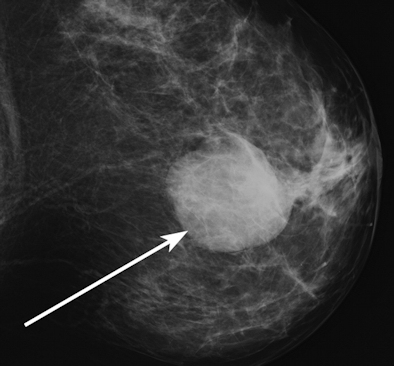
\includegraphics[width=0.75\textwidth]{masses.png}
\caption{\label{fig:frog}Mammographic image of a high-density mass (arrow)
}
\end{figure}

% Commands to include a figure:
\begin{figure}[!hbt]
\centering
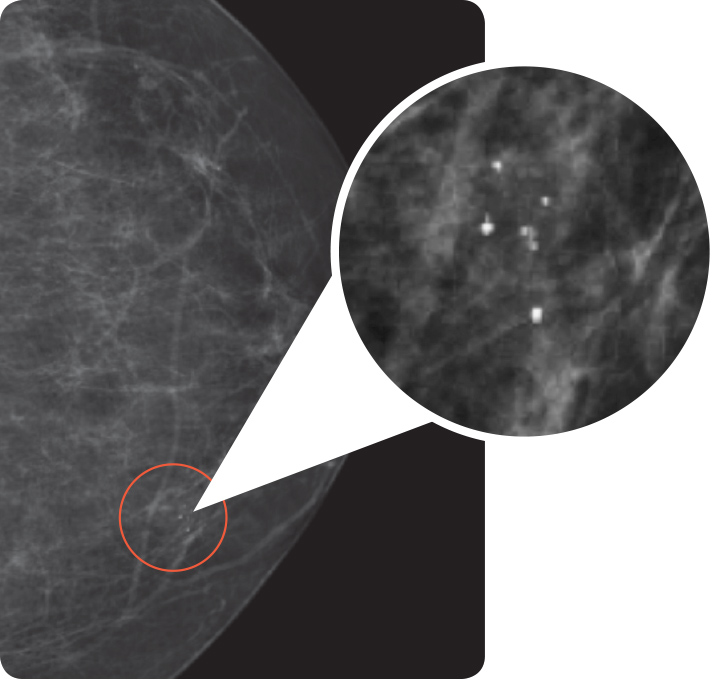
\includegraphics[width=0.75\textwidth]{calcifications.png}
\caption{\label{fig:frog}Mammogram – shows calcifications, an early sign of breast cancer
}
\end{figure}

\clearpage

\section{Introductory Related Work}

Some systems have been designed to provide more direct support for managing multiple concurrent activities associated with a large amount of digital material and tools. In our discussion below, we will follow clinical imaging tools and non-clinical imaging tools that propose for a multimodal and non-multimodal views.

\subsection{Activity-Based Computing}

For this paper report we approach many others like an Activity-Based Computing (ABC) for Medical Work in Hospitals [12] that presents the concept, which seeks to create computational support for human activities contributing to the growing research on support for human activities, mobility, collaboration, and context-aware computing. To sum up, activity-based computing builds and expands upon prior work within each of the areas described as activity management, virtual window management, collaboration support systems and context-awareness. However the last topics, it does not approach a multimodal view of images, but it was great on other fields of understanding the context and most of the problem/solutions.

\subsection{Fine Needle Aspirate}

By using computer based image analysing we research a Breast Cytology Diagnosis Via Digital Image Analysis [1] paper work that brings us an improvement on the diagnostic accuracy of breast fine needle aspirate (FNA) goal where an interactive computer system has been developed for evaluating cytologic features derived directly from a digital scan of breast FNA slides. The system uses computer vision technology techniques to analyse cell nuclei and classifies them using an inductive method based on linear programming.

\clearpage

The researched accuracy for medical imaging breast cancer diagnosis from FNAs varies considerably. Reported accuracy for visually diagnosing breast cancer from FNAs varies considerably. Giard and Hermans [13] researched on FNA performance parameters and found some sensitivities. The FNA diagnosis is highly operator-dependent and emphasised the need for developing individual performance characteristics for those doing this test. One goal of the present work is to improve the diagnostic accuracy of FNA by increasing its objectivity and thereby making it less operator-dependant. This image analysis and machine learning applied to breast cancer diagnosis and prognosis [14] study introduce us to a breast cancer diagnosis and prognosis by computer and to the value of aspiration cytologic examination of the breast into a statistical review of the medical literature [13].

\subsection{Picture Archiving and Communication Systems}

Medical services in current-time rely heavily on digital imaging technology due to image modalities utilised in medical field such as the computer Ecography, Mamography and Magnetic Resonance Imaging (MRI). These techniques require image-processing tools and digital management that has been the primary reason for development of Picture Archiving and Communication Systems (PACS) [15]. This technology provides economical storage and convenient access to images from multiple modalities where images are transmitted digitally via PACS where it eliminates the need to manually file, retrieve, or transport film jackets. The universal format for PACS image storage and transfer is Digital Imaging and Communications in Medicine (DICOM) [16] format.

A paper talking about web based medical images, data processing and management systems, present an application of database and functional imaging [17] that runs through the network and internet browser that has similar ability to the PACS yet having the advantages of being an online system can be viewed as archiving one step closer towards total online medical imaging system and online imaging in general. Despite the excellent information that this paper offer in the field of this research, we are more concerned with analysing the problem in a multimodality shed of image and interface surround, than this distribution of information side.

\subsection{Computer Aided Diagnosis}

The Picture Archiving and Communication System (PACS) [15] faces ever-growing adoption in hospitals and clinics worldwide [18] as we seen before. Digitalisation process and sharing of medical images is progressively replacing the use of tomography films, thus reducing costs and increasing the possibility of remote medical diagnosis through telemedicine solutions. Inline with this trend, Computer Aided Diagnosis (CAD) [19] is also gaining ground. CAD is an interdisciplinary technology combining elements of machine learn and computer vision with radiological image processing. A typical application is the detection of a tumor. For instance, some hospitals use CAD to support preventive medical check-ups in mammography (diagnosis of breast cancer). CAD typically intends to provide suggested diagnosis based on automatic quantitative analysis of medical images in order to aid physicians in their final diagnosis.

The computer suggested output may be useful in situations where the human visual system might fail or in case of fatigue of the physicians, alerting on possible well-known problems. According to a computer-aided diagnosis in medical imaging article [20], there are two CAD system types. The first type of CAD system assists with lesion detection, searching for abnormal standards in images like micro-calcifications groups in mammography images. The second type of CAD system assists the diagnosis, analysing the quantification of image characteristics where extracting information about a lesion shape may help to determine if a tumor is malignant or benign.

\clearpage

\section{Mobile Devices}

Mobile devices are increasingly being incorporated (Figure 3) onto Picture Archiving and Communication Systems (PACS). Previous work on medical image access using mobile devices essentially focuses on enabling the visualisation of the medical images at the mobile devices. In contrast, it can be proposed and developed a distributed system that allows medical image analysis using mobile devices. As a proof-of-concept, based on a mobile distributed system [20], which article develop a tool for dental implant simulation using mobile devices. There is also a discussion about the perspectives of extending the current system to incorporate Computer Aided Diagnosis (CAD) algorithms in it.

% Commands to include a figure:
\begin{figure}[!hbt]
\centering
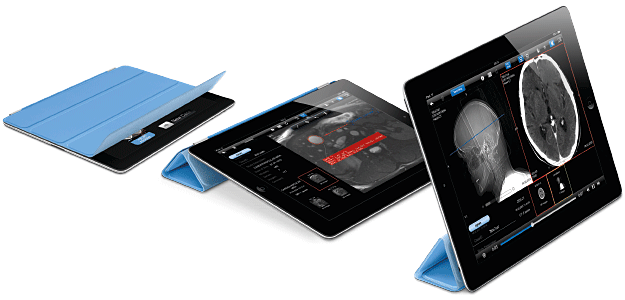
\includegraphics[width=0.75\textwidth]{mobile.png}
\caption{\label{fig:frog}aycan mobile
}
\end{figure}

Recently, mobile devices, such as PDAs, are being increasingly incorporated to PACS. Typically the flexibility on the visualisation of medical images storage in PACS, offered by a mobile access, is useful in patient care areas and emergency situations. This feature helps healthcare practitioners to have access to medical images at least for a preliminary image analysis in cases where searching for a dedicated terminal to access the images for a detailed and complete analysis is neither practical nor feasible.

The research proposes a distributed system that enables medical image analysis using mobile devices, as well as, the growth in the CAD area combined with the increase in processing power of the mobile devices and in the capacity of wireless networks favours the emergence of new developments integrating those technologies.

The communication between the mobile devices and the image server adopts web service technology [21]. To validate the distributed system processing power, speed, and feasibility we develop a tool for medical image analysis with mobile devices dedicated to assist in breast cancer visualisation diagnosis.

The deployed simulation tool allows the medic using a mobile device such as a PDA to determine the evolution of a patient like masses and calcifications location, preventing for instance the need for the doctor to move from analysis machine to the computer. After determine some critical areas, the doctor can visualise the analyse model of the result also using the mobile device. Results show that the use of mobile devices in hospital environments to assist the diagnosis and patient treatment is feasible. Other observation is that the mobile devices can be used to other tasks, like image model rendering, not only image visualisation.

\section{Conclusions}

There is a lot of information concerning work in development for clinical user interfaces on images tools views, but, in fact, there is little in multimodality image and its display in breast cancer diagnosis fields.

This article is a first essay, of many, to what will be the master thesis related work dissertation and state of the art [22]. It describe related systems that have been designed to provide more direct support and fundament to our research. We follow at most clinical imaging tools and personal computer-based interfaces as well as a hypothetical solution of implementation with mobile interfaces where it can help us understand the right user interface solution.

In short, we analyse and rehearsed what was the first approach to the subject-matter literature on a state of the art milestone of the project to understand and to investigate the various innovations and topics made in this field of research.

\clearpage

\begin{thebibliography}{}
\bibitem{} William H. Wolberg, W. Nick Street, Olvi L. Mangasarian. 1993. Breast Cytology Diagnosis. \emph{Via Digital Image Analysis}.
\bibitem{} Bennett KP, Mangasarian OL. Robust linear programming discrimination of two linearly inseparable sets. \emph{Optimization Methods and Software 1:23-34}, 1992.
\bibitem{} Mangasarian OL. Multi-surface method of pattern separation. \emph{IEEE Transactions on Information Theory IT-14:801-807}, 1968.
\bibitem{} Wolberg WH, Mangasarian OL. 1992. Multisurface method of pattern separation for medical diagnosis applied to breast cytology. \emph{Proceedings of the National Academy of Sciences}. U.S.A. 87:9193-9196.
\bibitem{} CZERWINSKI, M., HORVITZ, E., AND WILHITE, S. A diary study of task switching and interruptions. \emph{Proceedings of the Conference on Human Factors in Computing Systems}. ACM Press, 175–182.
\bibitem{} ROBERTSON, G., HORVITZ, E., CZERWINSKI, M., BAUDISCH, P., HUTCHINGS, D. R., MEYERS, B., ROBBINS, D., AND SMITH, G. Scalable fabric: Flexible task management. \emph{Proceedings of the Working Conference on Advanced Visual Interfaces}. ACM Press, 85–89.
\bibitem{} ROBERTSON, G., VAN DANTZICH, M., ROBBINS, D., CZERWINSKI, M., HINCKLEY, K., RISDEN, K., THIEL, D., AND GOROKHOVSKY, V. 2000. The task gallery: a 3d window manager. \emph{Proceedings of the SIGCHI Conference on Human Factors in Computing Systems}. ACM Press, 494–501.
\bibitem{} SMITH, G., BAUDISCH, P., ROBERTSON, G. G., CZERWINSKI, M., MEYERS, B., ROBBINS, D., AND ANDREWS, D. 2003. Groupbar: The taskbar evolved. \emph{Proceedings of the Australian Computer-Human Interaction Special Interest Group (OZCHI)}.
\bibitem{} BARDRAM, J. E. AND CHRISTENSEN, H. B. 2004. Real-time collaboration in activity-based architectures. \emph{Proceedings of 4th Working IEEE/IFIP Conference on Software Architecture (WICSA ’04)}. IEEE Press, 325–329.
\bibitem{} GONZALEZ, V. M. AND MARK, G. 2004. “Constant, constant, multi-tasking craziness”: Managing multiple working spheres. \emph{Proceedings of the SIGCHI Conference on Human Factors in Computing Systems (CHI ’04)}. ACM Press, 113–120.
\bibitem{} MARK, G., GONZALEZ, V. M., AND HARRIS, J. 2005. No task left behind?: Examining the nature of fragmented work. \emph{Proceedings of the SIGCHI Conference on Human Factors in Computing Systems (CHI ’05)}. ACM Press, 321–330.
\bibitem{} BARDRAM, J. E. 2009. Activity-Based Computing for Medical Work in Hospitals. \emph{ACM Transactions on Computer-Human Interaction}.
\bibitem{} Giard RWM, Hermans J. 1992. The value of aspiration cytologic examination of the breast. A statistical review of the medical literature. \emph{Cancer.69:2104-2110}.
\bibitem{} William H. Wolberg M.D. W. Nick Street M.S. and Olvi L. Mangasarian Ph.D. 2009. Activity-Based Computing for Medical Work in Hospitals. \emph{ACM Transactions on Computer-Human Interaction}.
\bibitem{} Oosterwijk, Herman. 2004. PACS Fundamentals. \emph{Aubrey: OTech Inc}. ISBN 978-0-9718867-3-5.
\bibitem{} Mustra, Mario; Delac, Kresimir; Grgic, Mislav. September, 2008. Overview of the DICOM Standard. \emph{ELMAR, 2008. 50th International Symposium. Zadar, Croatia}. pp. 39–44. ISBN 978-1-4244-3364-3.
\bibitem{} Jinman Kim, David D. Feng, Tom W. Cai. 2000. A Web Based Medical Image Data processing and Management System. \emph{Conferences
in Research and Practice in Information Technology}. Vol. 2.
\bibitem{} H. U. Lemke. PACS developments in Europe. \emph{Computerized Medical Imaging and Graphics}, 27:111–120, 2003.
\bibitem{} Maryellen L. Giger; Nico Karssemeijer. September, 2008. Computer-Aided Diagnosis. \emph{Proceedings of SPIE}. 1605-7422, v. 6915.
\bibitem{} B. Correa, E. Ishikawa; A. Ziviani; M. Faria. 2008. Medical Image Analysis using Mobile Devices. \emph{SAC’08 March 1620, 2008, Fortaleza, Cear´a, Brazil}. ACM 9781595937537/08/0003.
\bibitem{} Web Service. Electronically available information at. \emph{http://www.w3.org/2002/ws/}.
\bibitem{} Timothy Borchers. Persuasion in the Media Age: \emph{Third Edition (2012)}, p. 85.
\end{thebibliography}

\end{document}
